%-----------------------
% Title page
%-----------------------
\begin{titlepage}
    \centering

    \textsc{ELEC4630 Assignment 1}\\
    \vspace{9cm}

    \rule{\linewidth}{0.5pt}\\

    \vspace{1em}
    \LARGE\textsc{Question 1}\\
    \vspace{1em}

    \LARGE\uppercase{\textbf{{Road Sign Segmentation}}}\\

    \rule{\linewidth}{2pt}\\

    \vfill

    \normalsize{Deren Teo (4528554)}
    \vspace{1cm}

\end{titlepage}

%-----------------------
% Report body
%-----------------------
\section{Introduction}

Road sign detection is an important aspect of the advanced driver assistance systems found in most modern road vehicles, and is essential to achieving autonomous driving. Yet, it is a reasonably challenging task for traditional computer vision techniques, due to the wide variety of road sign shapes, sizes, colours and possible viewing angles. Furthermore, adverse lighting conditions, weather-impeded visibility and partial obstruction present further difficulties to detection. This report presents a simple approach to road sign detection using template matching. It successfully detects a variety of signs, but is non-robust against non-Euclidean transforms and adverse lighting, in particular.

\section{Background Theory}

\subsection{Template Matching}

Template matching is a technique used to identify the location of a template in a larger image \cite{opencv_tm}. The process involves a 2D convolution of the template with an image; for each pixel in the image, a value is calculated indicating how well the neighbourhood of the pixel matches the template \cite{opencv_tm}. Several formulae are available for calculating this value \cite{opencv_tm}; however, this report focuses on normalised cross-correlation.

Normalised cross-correlation is defined as the inverse Fourier transform of the convolution of the Fourier transform of two images \cite{psi_2016}. The intuition of the values produced by this method is similar to the dot product between two normalised pixel intensity vectors \cite{psi_2016}. This method is used for the speed afforded by the Fourier transforms \cite{psi_2016}.

Normalised cross-correlation is based on the formula \cite{opencv_tm}:
\begin{align}
  R(x,y) = \frac{\sum_{x',y'}\left(T(x',y')\cdot I(x+x',y+y')\right)}{\sqrt{\sum_{x',y'} T(x',y')^2 \cdot \sum_{x',y'} I(x+x',y+y')^2}}
\end{align}
where $R(x,y)$ is the normalised cross-correlation value at pixel position $(x,y)$ in the image, $T(x',y')$ is a pixel in the template, $I(x+x', y+y')$ is a pixel in the image, and the denominator is the magnitude of the numerator.

The formula can be corroborated with the intuition by observing that for each pixel $(x,y)$ in the image, there is a sum over all the pixels $(x',y')$ in the template. This produces a metric of ``similarity'' between the template and the neighbourhood of pixel $(x,y)$ in the image. This is repeated for each pixel in the image, which can be intuitively understood as ``sliding'' the template over the image at each step.

The result is a surface of normalised cross-correlation values, where the highest peak in the surface indicates the highest cross-correlation and therefore the location of the best match between the template and the image.

\subsection{Chamfer System}

Gavrila \cite{gavrila_2007} \cite{gavrila_nd} presents an advanced template matching approach using a template tree and Bayesian model to optimise the matching of complex shapes, such as pedestrians, which may be observed in a wide range of sizes, poses and orientations. While Gavrila's Chamfer System \cite{gavrila_nd} is out of the scope of this report, one relevant technique it applies is the use of a blurring function to enable template matching on subjects very similar but non-identical to the template. This increases the flexibility of each template, and is useful to road sign detection given the wide variety of similar but non-identical signs. It is also useful in matching partially obstructed and angled signs.

\newpage
\section{Methodology}

This section summarises the approach used to detect road signs of varying color, size and shape. The approach is split into three distinct subsections: image processing to enhance red and yellow signs, image processing to enhance white signs, and template matching on the processed images.

The processing of red/yellow signs is separate from white signs because it is difficult to clearly separate both categories from a variety of backgrounds using the same technique. In particular, red/yellow signs stand out well in the saturation channel but white signs do not; meanwhile, white signs stand out better in grayscale, but red/yellow signs do not.

First, for processing images to enhance red/yellow signs:
\begin{enumerate}
  \item The image is converted to HSV and the saturation channel is extracted, since red and yellow signs consistently have high saturation.

  \item The image is blurred then thresholded to remove background details. Blurring before thresholding helps remove fine details, such as bright spots in the background.

  \item The image is morphologically dilated then opened, to join disconnected components before removing noise. This reduces the likelihood of important features being removed by the opening.

  \item Contours in the image are identified and filled. This aims to white out the black symbols inside the signs, enabling more consistent template matching with a solid template.

  \item Finally, the image is blurred to enable template matching of signs that are slightly angled or otherwise distorted.

\end{enumerate}

Then, for processing images to enhance white signs:
\begin{enumerate}
  \item The image is converted to grayscale and blurred using a bilateral filter to remove small background details while preserving sign edges.

  \item Two thresholds are used to binarize the image; a lower threshold removes most of the darker background, while an upper threshold removes bright sky.

  \item The binary image is morphologically eroded to disconnect foreground regions. This is in preparation for the flood fill in the following step, and makes it less likely that parts of signs are unintentionally removed.

  \item A black flood fill is applied to remove white areas connected to the image border. This aims to remove remaining large white areas of background without erasing sign details, and is particularly useful for removing remaining areas of sky.

  \item Finally, the image is blurred to enable template matching of signs that are slightly angled or otherwise distorted.

\end{enumerate}

Finally, template matching is used to detect signs in the processed images. Since red/yellow signs and white signs occur mutually exclusively in the processed images, a set of templates is defined for either class, encompassing the expected sign shapes for each respective colour.

\newpage

For red/yellow signs, the following templates are defined:

\begin{figure}[ht]
  \centering
  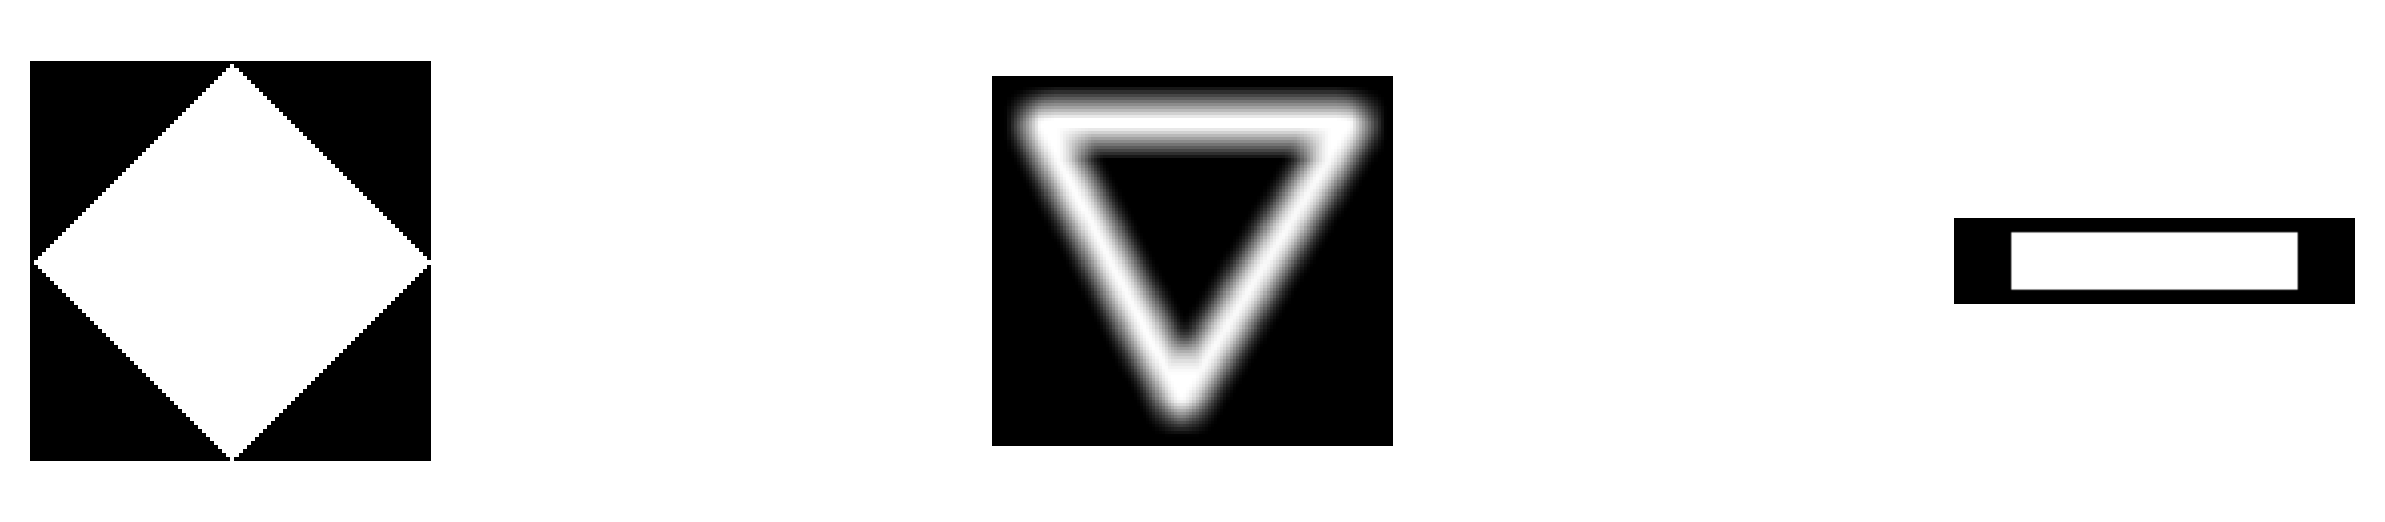
\includegraphics[width=0.7\textwidth]{images/q1_templates_a.png}
\end{figure}

For white signs, the following templates are defined:

\begin{figure}[ht]
  \centering
  
\includegraphics[width=0.7\textwidth]{images/q1_templates_b.png}
\end{figure}

Given a processed image and associated templates, the following process is then applied to detect signs:
\begin{enumerate}
  \item For each template, a range of scaling factors is defined to match the range of sign sizes present in the set of sample images. Problems with this approach are presented in the Discussion section.

  \item Each template is scaled through its range of possible sizes, and template matching is performed using each scaled template. The template matching applies normalised cross-correlation and an experimentally tuned threshold of 0.85.

  \item All matches are added to a list, recording the location, template size, and match value. The location and size of the templates do not include the black borders.

  \item Finally, overlapping matches are removed, prioritising those with the highest match value. The overlap is calculated using the match locations and template dimensions; if the overlap exceeds 15\% of the area of the smaller template, only the better match is retained.

\end{enumerate}

This procedure returns rectangles around each detected sign, as defined by the location and size of the best matching template. The rectangles can then be drawn onto the original image to observe the results of the detection.

\section{Results}

Figure \ref{fig:q1aresults} presents the results of the solution for the first sample image.

\begin{figure}[ht]
  \centering
  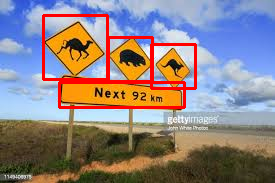
\includegraphics[width=0.4\textwidth]{images/q1_results_a.png}
  \caption{Detected signs in \texttt{images0.jpg}}
  \label{fig:q1aresults}
\end{figure}

\newpage

Figure \ref{fig:q1bresults} presents the results of the solution for the 10 other sample images.

\begin{figure}[ht]
  \centering
  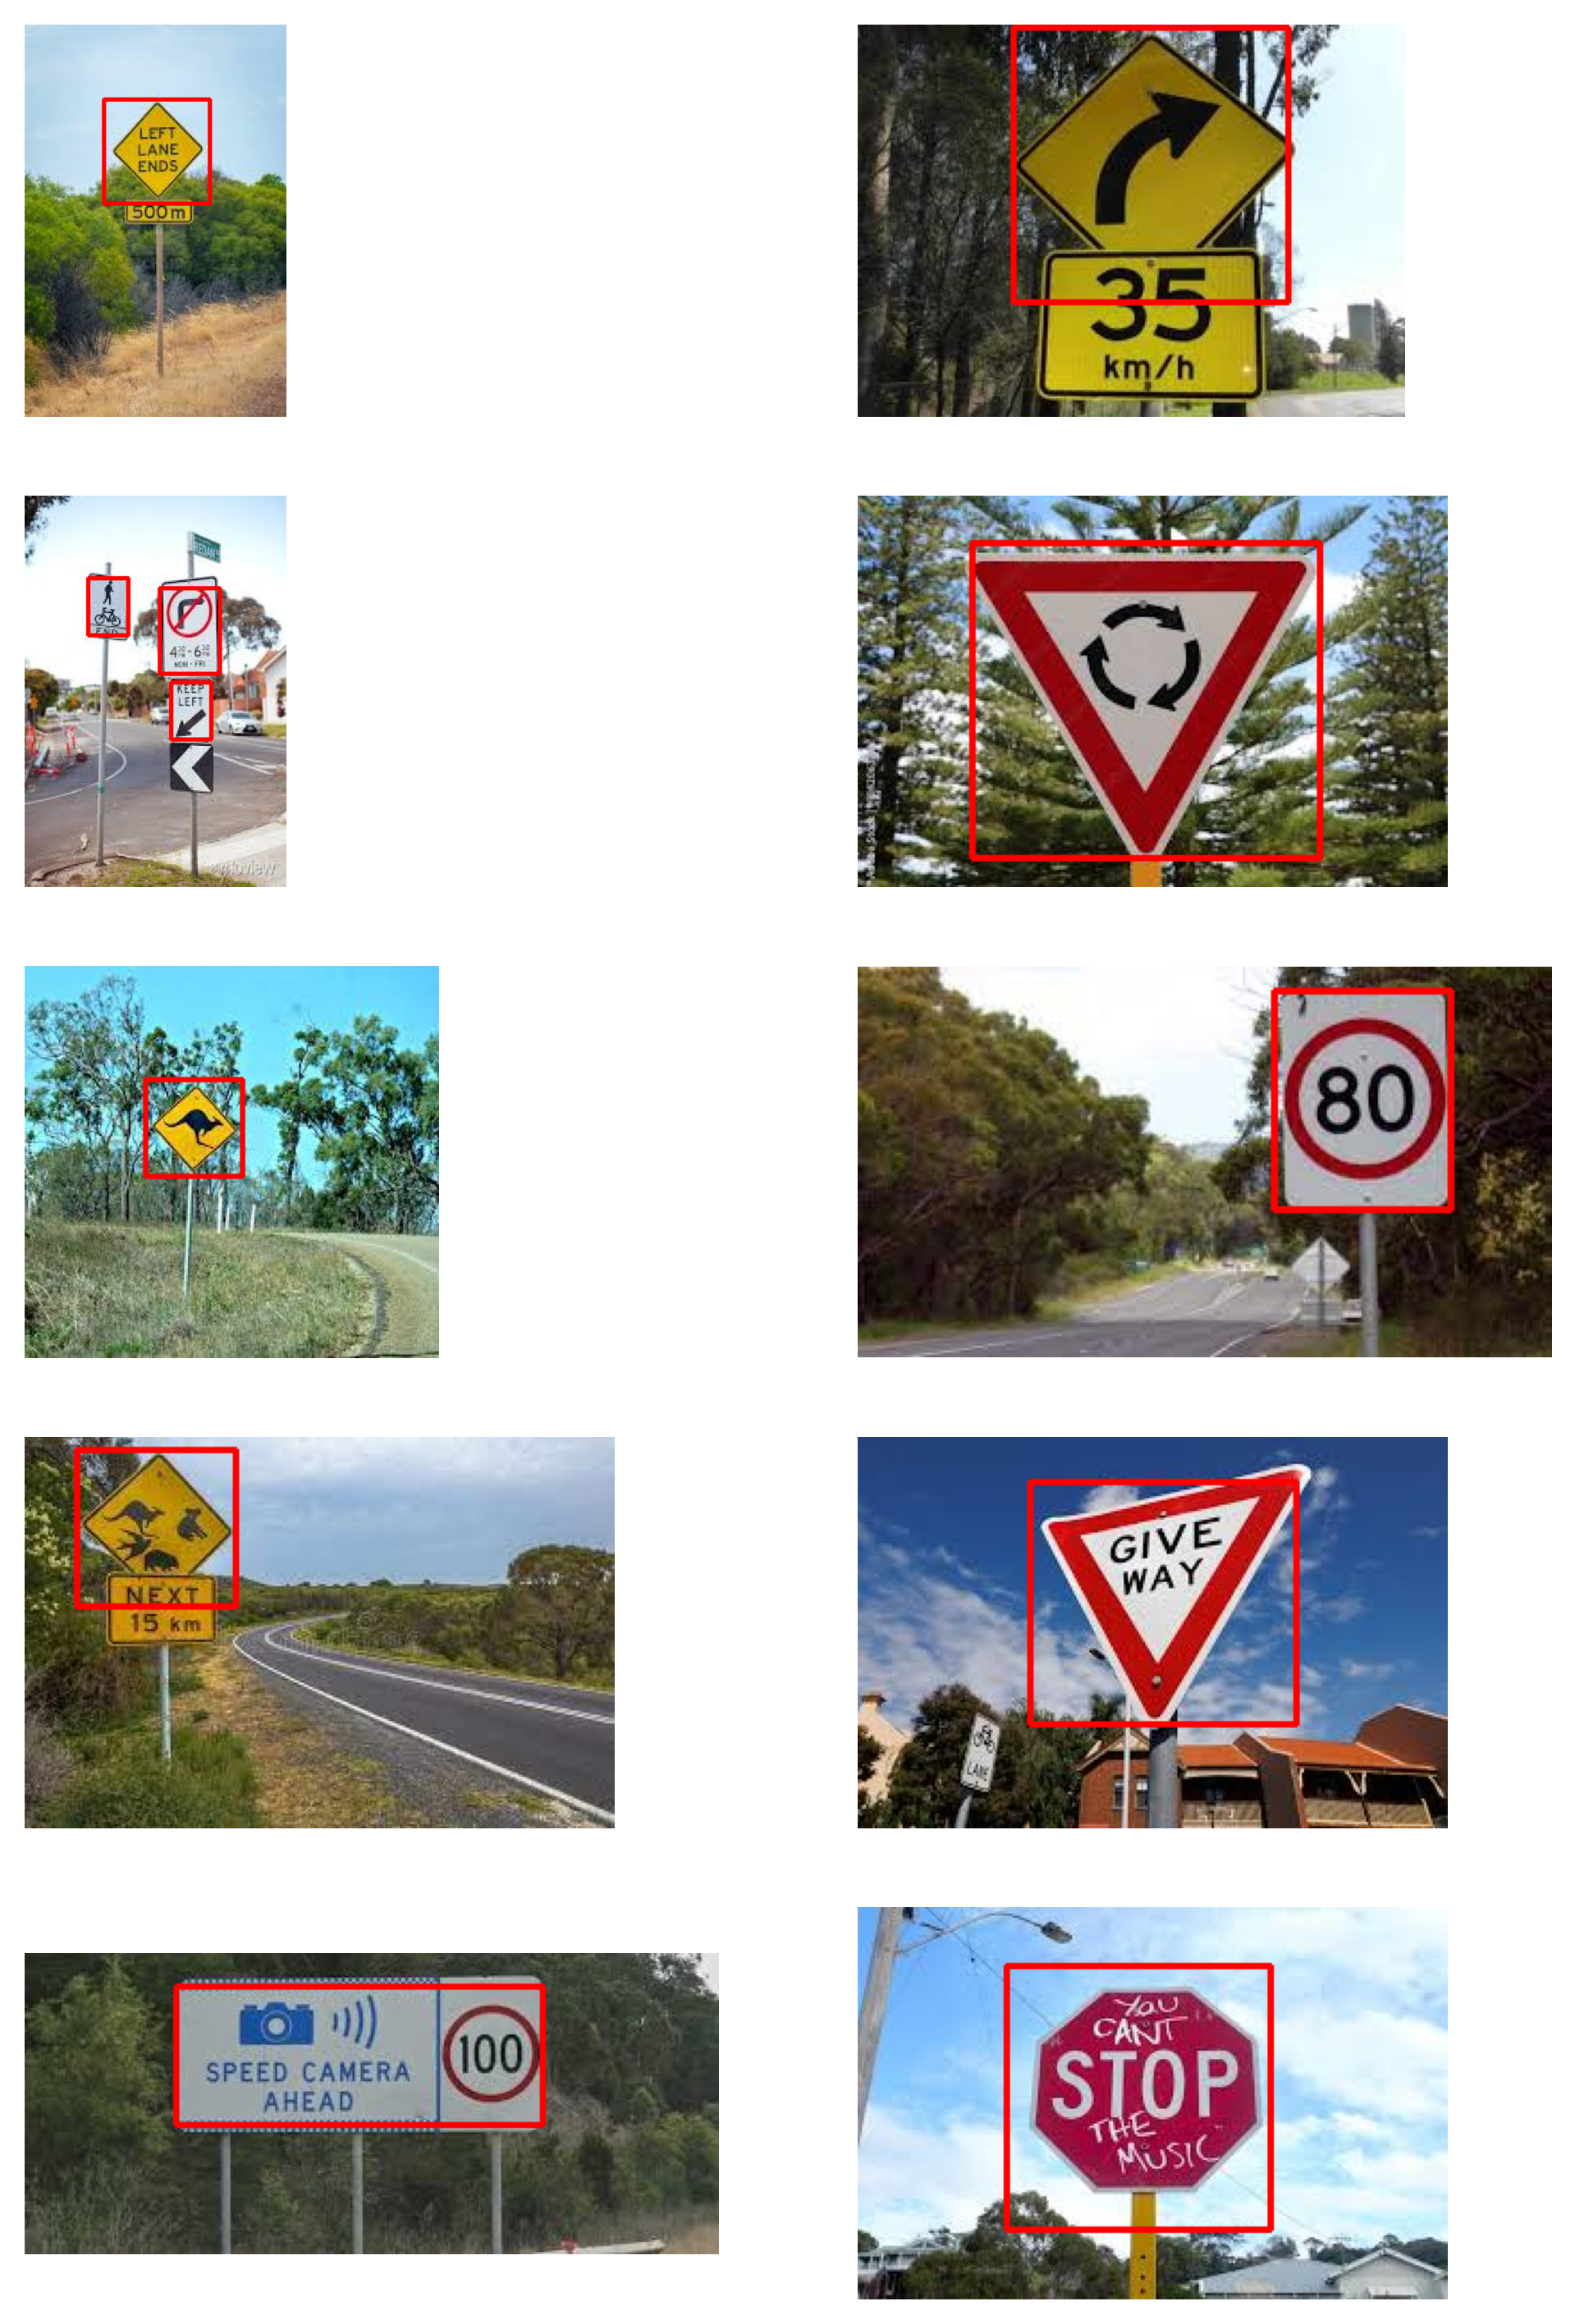
\includegraphics[width=0.78\textwidth]{images/q1_results_b.png}
  \caption{Detected signs in \texttt{images1.jpg} through \texttt{images10.jpg}}
  \label{fig:q1bresults}
\end{figure}

The solution detects all signs in the first image, but it has mixed success with the other ten images. Out of the 22 visible signs in all 11 images, 16 are detected, representing a detection rate of 73\%.

\newpage
\section{Discussion}

This report has presented a solution for detecting the position and size of various road signs in an image. The method successfully identifies 16 out of 22 signs in the sample set of 11 images. While this is a reasonable outcome, there remains significant room for improvement. Yet even so, the presented method already requires highly specific tuning of many parameters to maximise the detection rate across the samples; therefore, it is likely to generalise poorly to other images.

(Template shapes and scaling and limitations of template matching)

(Separating of red/yellow and white samples, and inability to do both)

(General difficulties with detecting road signs)

(Possible improvement: Gavrila Chamfer System)

\section{Conclusion}

In summary, this report presents a simple solution to the task of detecting road signs in images. The solution achives reasonble results on the sample set of images, identifying 73\% of visible road signs, though significant room for improvement remains. Caveats of the solution are discussed, largely surrounding the highly specific tuning required to achieve the presented results. The report concludes with a discussion on the common challenges in road sign detection, and possible improvements to the presented solution.
